%!TEX root = ../main.tex
\section{Hardware implementation}
The group was given 2 Pittman 9234 24V motors, the models being 9234S007-R1 and 9234S006, a dual H-bridge and a dSPACE system.
The Pittman 9234S007 is equipped with a rotational encoder.
The dSPACE system is connected to the H-bridge which drives the motors. 
The setup can be seen in figure~\ref{fig:implementation_block}.
Furthermore, the encoders of the motor are connected to the dSPACE system.
A Lecroy wavesurfer 3054 oscilloscope with current probes and KE 34310A multimeters are used in the experiments conducted throughout the report.

\begin{figure}[!h]
\centering
%!TEX root = ../main.tex

%\documentclass{standalone}

%\usepackage{tikz}

% The block diagram code is probably more verbose than necessary
\begin{tikzpicture}[auto, node distance=3.5cm,>=latex']
    % We start by placing the blocks
    \node [block] (motor) {Motors};
    \node [block, left of=motor] (hbro) {H-bridge};
    \node [block, left of=hbro] (dspace) {dSPACE};
    \node [block, right of=motor] (encoder) {Encoders};
    \node [below= 1cm of motor] (point) {};
    \node [above= 1cm of motor] (point1) {};
    \node [blockg, right =0.5cm of point1] (scope) {Oscilloscope};
    \node [blockg, left =0.5cm of point1] (multi) {Multimeter};


    \draw[->] (hbro) -- (motor);
    \draw[->] (dspace) -- (hbro);
    \draw[->] (motor) -- (encoder);
    \draw[->] (motor) -- (encoder);
    \draw[-] (encoder) |- (point.west);
    \draw[->] (point) -| (dspace);
    \draw[->] (motor) |- (scope);
    \draw[->] (motor) |- (multi);


  %\node[label=above:C] (C)  [below right=0.7cm and 4cm of B1]
   %    {($2m-1$)};
    %\draw [draw,->] (input) -- node {$r$} (sum);
    %\draw [->] (sum) -- node {$e$} (controller);
    %\draw [->] (system) -- node [name=y] {$y$}(output);
    %\draw [->] (y) |- (measurements);
\end{tikzpicture}

%\end{document}


  \caption{Block diagram showing the motor setup.}
  \label{fig:implementation_block}
\end{figure}

The dSPACE system was setup with a low sampling time, $T_s$, in order to avoid oversampling the encoder inputs.
$T_s$ was choosen to be 1kHz. 
The hardware setup of the encoder input and the PWM output can be seen in figure \ref{fig:encoder} and \ref{fig:pwm}, respectively.


\begin{figure}[!h]
\centering
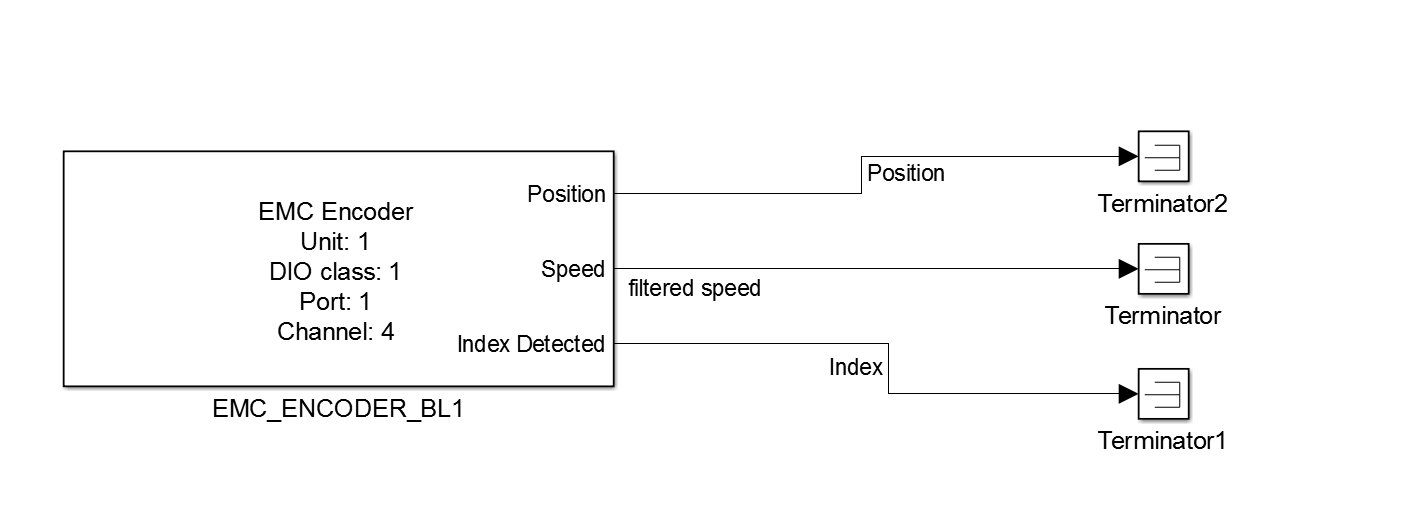
\includegraphics[scale=0.3]{graphics/encoder.png}
  \caption{Encoder setup in dSPACE.}
  \label{fig:encoder}
\end{figure}

\begin{figure}[!h]
\centering
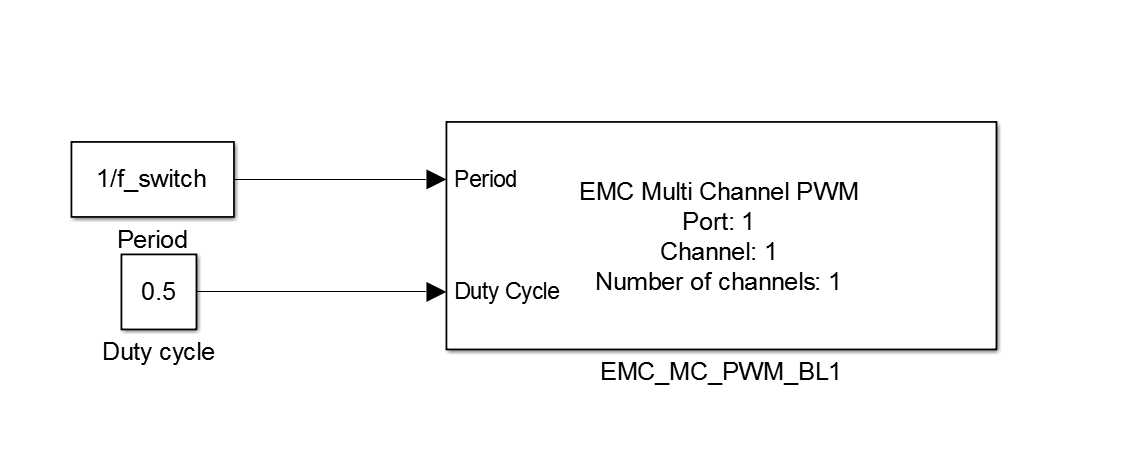
\includegraphics[scale=0.3]{graphics/pwm.png}
  \caption{PWM setup in dSPACE.}
  \label{fig:pwm}
\end{figure}

\todo{Add paragraph about dSpace setup - Mikkel}